
\section{Transfer Learning}
\label{sec:InfoForPrediction}

\subsection{The need for contact models}
The input domains of $f$, $f_{qs}$, and $p_{qs}$ are insufficient to pose problems P2 (Action Transfer) or P3 (Shape Transfer). This is because they only capture the {\em global} relations between objects. To properly pose transfer learning, the input domain must capture all the {\em local} contact relations between the object and its surroundings.  To see why consider Figure~\ref{fig:Learning.shapes}. On the left is a training example. On the right is a test case, where the object is wider. Given the same placement of the frames on object and agent, and the same finger motion, the predicted behaviour using Equation~\eqref{eq:Learning.short} will be the same as for the training example. This is wrong. For the correct prediction to be transferred, additional information is needed about the contact between $A$ and $B$. This can be captured by attaching additional frames to $A$ and $B$ close to their point of contact (see Figure~\ref{fig:Learning.setup2}, centre panel).

In general, an object has multiple contacts with the robot and the environment. Each of these contacts provides a kinematic constraint on the object's motion, and thus each one should be modelled. Rigid body simulators use just such contact information.

\subsection{Modelling contacts and near contacts} 
We use a pair of local frames to encode each contact or near contact. Each pair encodes a transformation between part of the object $B$ and another body.  To distinguish these local frame pairs from what has gone before we henceforth refer to the main frame attached to a body (defined in Section~\ref{sec:Representations}) as that body's global frame. We define the local frame pairs as follows. Consider Figure~\ref{fig:Learning.setup2}  (left panel). We first define a pair of local frames capturing the finger-object contact as $A^{L}_{t}$ and $B^{L}_{t}$ (centre panel). These are spatially dynamic, i.e.\ at any time $t$ they are located at the points of closest proximity on the finger and object respectively.  We define the \textit{agent-object contact}
information as the transformations $T^{A^{L}_{t}, A^{L}_{t+1}}$ and $T^{A^{L}_t, B^{L}_t}$.

We also define local frame pairs, to model object-environment contacts. One frame is attached to some point on the object ($B^{Sk}_t$), and one is attached to the nearest point in the environment $E^{Sk}_t$.  Thus the environment frame within each pair is spatially dynamic, changing its position as the object moves. If $N$ points on the object are chosen for modelling there will be $N$ pairs of local frames $B^{Sk}_t$ and $E^{Sk}_t$ to capture the object-environment contacts at time $t$, where ($k=1 \ldots N$) (Figure~\ref{fig:Learning.setup2} right panel). Using these frame pairs, we then define the \textit{object-environment contact} information as the set of transformations $T^{E^{Sk}_t,B^{Sk}_t}$ for $k=1 \ldots N$. 

This section described the information required to allow transfer learning. We refer to this as {\em contact} information, even though it also includes information on surfaces not in, but close to, contact. 

\subsection{Learning a contact model}
Given observations of moving surfaces in contact, and near contact, it is possible to learn contact models. In this paper, during training, two contact models are learned: an agent-object contact model, and an object-environment contact model. The object-environment contact model is created by pooling data from frames located at several points on the object. Thus, a learned model of contact behaviour is created from many contact examples. This contrasts with the analytic approach used by rigid body simulators. An extension would be to condition this model on other variables, for example information on local surface properties, such as shape or texture. We hypothesize that both data pooling and conditioning will be important elements in improving the transfer of predictions. 

\begin{figure}[t]
\centerline{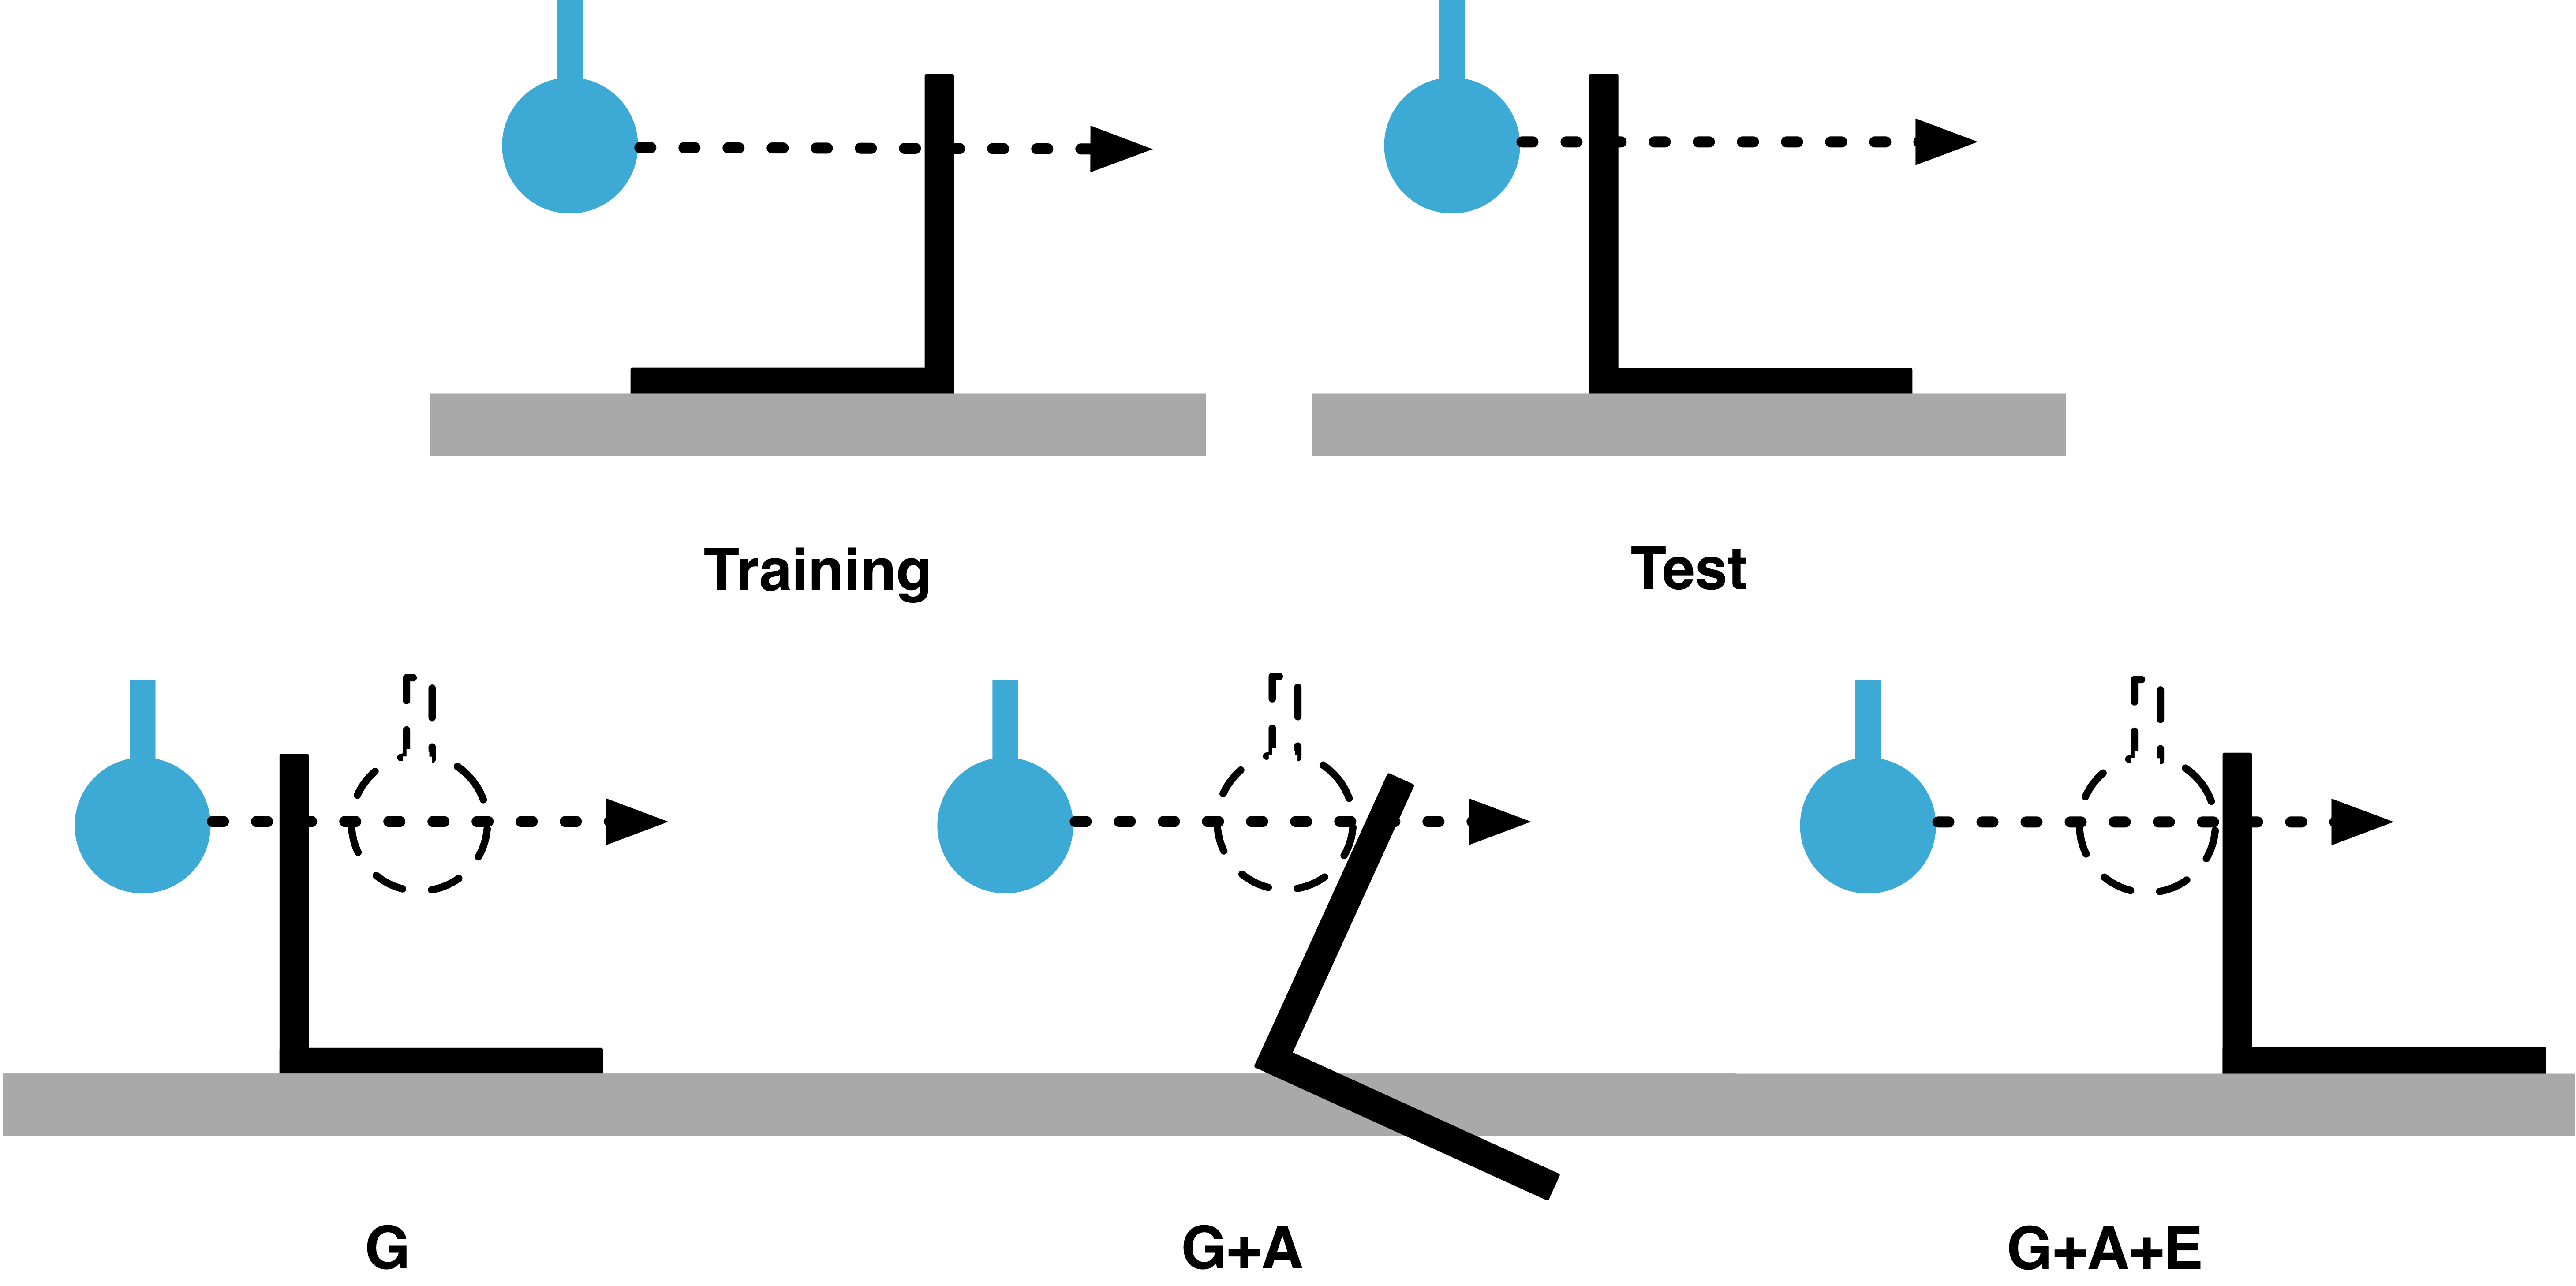
\includegraphics[width=\columnwidth]{BackPushToyExample}}
\caption[ToyExample]{Information for Action Transfer: an L-shaped object is pushed by a finger. Various predictors are trained solely on forward pushes (top left), but tested on backwards pushes (top right). The top panels show a training and a test push, whereas the bottom panels show predictions given different information (G, G+A and G+A+E) for the test push.}
\label{fig:ToyExample}
\end{figure}

\subsection{Predicting with contact models}
During transfer the learned contact models are applied. One issue is how we map the various references frames from the training examples to the test examples. For problems P1 and P2 this is trivial, since the objects are the same. For problem P3 this is done partly by the experimenter, and partly algorithmically. The global frame is attached to a representative central point on the object. An object-environment frame, $B^{Sk}_t$, is attached to a central point on each surface segment with constant curvature. This strategy was determined empirically. The object-environment expert, since it is trained on a mixture of contact behaviours, is robust to a variety of placements. 
Each expert is a copy of the single, learned object-environment model. Thus several, identical, contact experts are created on the new object. How to fully automate the placement strategy for P3 remains an open question. Finally, we note that we have motivated these contact experts as enabling shape transfer, but they are equally applicable to action transfer. The top row of Figure~\ref{fig:ToyExample} shows a training and a test case for problem P2 (action transfer). The prediction for the test case requires encoding of the kinematic constraint imposed by the contact between the base of the L-shaped flap and the table. This constraint also existed in the training push, but was not significant since the flap could rotate on its corner.

\subsection{Hypothesized benefits of contact modelling}
We can now consider the effects that different sets of information might have. We shall refer to a predictor that uses only the global frames, $A$ and $B$, as having global information (G). We can add agent-object contact information (G+A), and object-environment contact information (G+A+E). Now consider the possible predictions for the test case (Figure~\ref{fig:ToyExample} bottom row). A predictor using G will predict that the object will not move. A predictor using G+A has information, from the training case, that the object surface will move with the finger, so that the finger will not pass through it. But this information is also capable of predicting that the object rotates about the corner and into the table, since it doesn't model the object-environment contact. A predictor using G+A+E will have information about the effect of the contact between the base of the flap and the table, and so should avoid predicting a rotation into the table.
One point is critical, this analysis only concerns what the information allows. Performance will depend on a learner's ability to utilise it.  

\subsection{Reformulating prediction with contact information}
We can simply extend the prediction formulations to incorporate contact information. For regression we simply enlarge the domain of function~$f$
in Equation~\eqref{eq:Learning.short}:
\begin{multline}
f'_{qs}: T^{A_t, B_t}, T^{B_t, O}, T^{A_{t}, A_{t+1}}, T^{A^{L}_t, B^{L}_t} \\ \{, T^{E^{Sk}_t,B^{Sk}_t}\}_{k=1 \ldots N} \longrightarrow T^{B_{t}, B_{t+1}}
\label{eq:Learning.augmented}
\end{multline}
Recall that, at prediction time, we will need $N$ copies of the object-environment contact information, which was pooled at the learning stage. Hence, we use $k$ to index over these copies. Unfortunately, because the dimensionality of the domain of $f'_{qs}$ grows with the number of environment contacts, $N$, the difficulty of learning the mapping $f'_{qs}$ rapidly increases as environment contacts are added.

The conditional probability density (CPD) $p_{qs}$ over possible object motions $T^{B_{t}, B_{t+1}}$~\citep{kopicki_prediction_2009} is augmented as follows:
\begin{multline}
p_{qs}(T^{B_{t}, B_{t+1}} | T^{A_t, B_t}, T^{B_t, O}, T^{A_{t}, A_{t+1}}, T^{A^{L}_t, B^{L}_t} \\ \{, T^{E^{Sk}_t,B^{Sk}_t}\}_{k=1 \ldots N})
\label{eq:Learning.density}
\end{multline}

Again the dimensionality of the conditioning variables makes density estimation hard as the number of contacts grows. One way around this, in the density estimation case, is to factorize the density in a way that reflects the contact structure. We consider this in the next section.